%\section {Définitions}

%
%  Configuration space
%

\begin{frame} {Configuration space}
  \centerline {
    \parbox{.7\linewidth} {
      Configuration
      \begin{eqnarray*}
        &&\conf=(\conf_{r_1},\conf_{r_2},\conf_{c_1},\conf_{c_2},\conf_{s_1},\conf_{s_2}) \\
        &&\conf_{r_1}, \conf_{r_2}\in\real^6 \\
        &&\conf_{c_1},\conf_{c_2},\conf_{s_1},\conf_{s_2}\in\real^7
      \end{eqnarray*}
      where
      \begin{eqnarray*}
        &&\conf_{r_1} = (q1,\cdots,q_6) \mbox{ is the vector of joint angles,} \\
        &&\conf_{c_1} = (x, y, z, X, Y, Z, W) \\
        &&W + Xi + Yj + Zk \mbox{is a \textbf{unit} quaternion}.
      \end{eqnarray*}
      The configuration space is a differential manifold.
    }
    \parbox {.39\linewidth} {
      \centerline {
        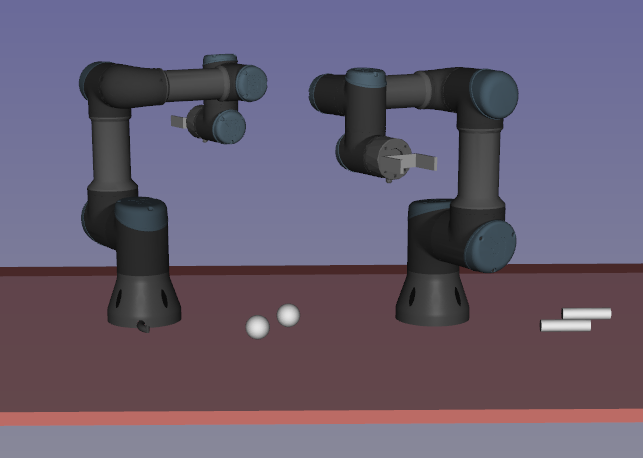
\includegraphics[width=\linewidth]{figures/configuration-space.png}
      }
      \vskip 5cm
    }
  }
\end{frame}

%
%  Quaternion
%
\begin {frame} {Quaternions}
  \centerline {
    \parbox {.75\linewidth} {
      Non-commutative field isomorphic to $\real^4$, spanned by three elements
      $i, j, k$ that satisfy the following relations~:
      $$i^2 = j^2 = k^2 = ijk = -1$$
      \pause
      from which we immediately deduce
      $$ ij=k,\ jk=i,\ ki=j$$
    }
    \parbox {.24\linewidth} {
      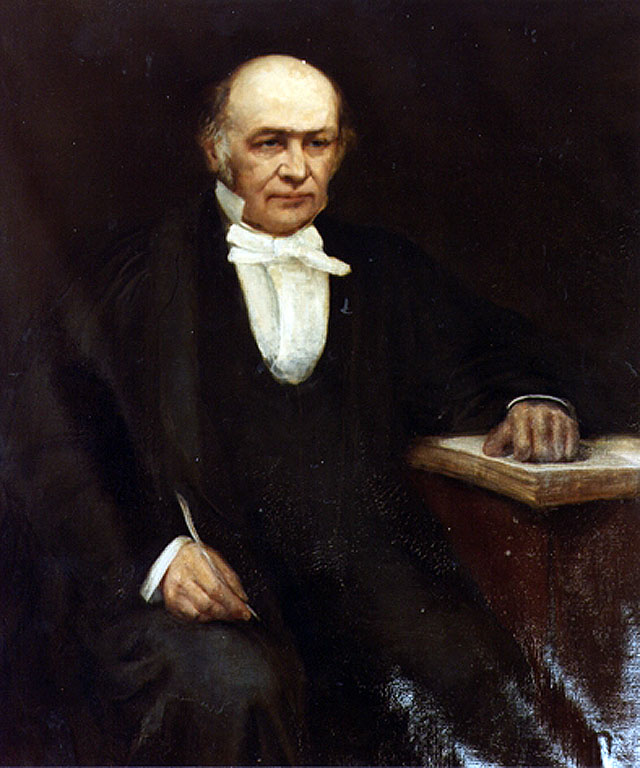
\includegraphics [width=\linewidth] {figures/William_Rowan_Hamilton_painting.jpg}\\
      \centerline {Hamilton (1843)}
    }
  }
\end {frame}

%
%  Quaternions unitaires et rotations
%
\begin {frame} {Unit Quaternions and rotations}
  Let $q=q_0 + q_1 i + q_2 j + q_3 k$ be a unit quaternion:
  $$q_0^2 + q_3^2 + q_2^2 + q_3^2 = 1$$
  \pause
  $\forall x = (x_0, x_1, x_2)\in\real^3$, let $u=x_0i + x_1 j + x_2 k$
  $$
  q\,.\,u\,.\,q^* = y_0 i + y_1 j + y_2 k
  $$
  where $q^*=q_0 - q_1 i - q_2 j - q_3 k$ is the conjugate of $q$.\\
  \pause
  $y = (y_0, y_1, y_2)$ is the image of $x$ by the rotation of matrix
  $$
  \left(\begin{array}{ccc}1 - 2(q_2^2 + q_3^2) & 2q_2q_1 - 2q_3q_0 & 2q_3q_1 + 2q_2q_0\\ 2q_2q_1 + 2q_3q_0 & 1 - 2(q_1^2 + q_3^2) & 2q_3q_2 - 2q_1q_0\\ 2q_3q_1 - 2q_2q_0 & 2q_3q_2 + 2q_1q_0 & 1 - 2(q_1^2 + q_2^2)\end{array}\right)
  $$
\end{frame}

%
%  Quaternions unitaires et rotations
%
\begin {frame} {Unit Quaternions and rotations}
  \begin{itemize}
    \item Notice that $q$ and $-q$ represent the same rotation
  \end{itemize}
\end{frame}

%
%  Obstacle
%

\begin{frame} {Definitions}

\begin{itemize}
\item Workspace: $\WS=\real^2$ or $\real^3$: space in which the robot evolves
\pause
\item Obstacle in workspace: compact subset of $\WS$, denoted by $\obst$.
\pause
\item Configuration space: $\CS$.
\pause
\item Position in configuration $\conf$ of a point $M\in\body_i$:
  $\x_i(M,\conf)$.
\pause
\item Obstacle in the configuration space:
\begin{eqnarray*}
\CSobst&=\{\conf\in\CS,&\exists i\in\{1,\cdots,m\},\ \exists M\in\body_i,\ \x_i(M,\conf)\in\obst\ \mbox{or}\\
&&\exists i,j\in\{1,\cdots,m\},\ \exists M_i\in\body_i,\ \exists M_j\in\body_j,\\
&&\x_i(M_i,\conf)=x_j(M_j,\conf)\}
\end{eqnarray*}
\pause
\item Free configuration space: $\CSfree = \CS\setminus\CSobst$.
\end{itemize}
\end{frame}

%
%  Motion
%

\begin{frame} {Motion}

\begin{itemize}
\item Configuration space:
  \begin{itemize}
  \item differential manifold
  \end{itemize}
  \pause
\item Motion:
  \begin{itemize}
  \item continuous function from $[0,1]$ to $\CS$.
  \end{itemize}
  \pause
\item Collision-free motion:
  \begin{itemize}
  \item continuous function from $[0,1]$ to $\CSfree$.
  \end{itemize}
\end{itemize}
\end{frame}

%
%  Motion planning
%

\begin{frame} {Motion planning problem}
  \parbox{.49\linewidth}{
    \centerline{
      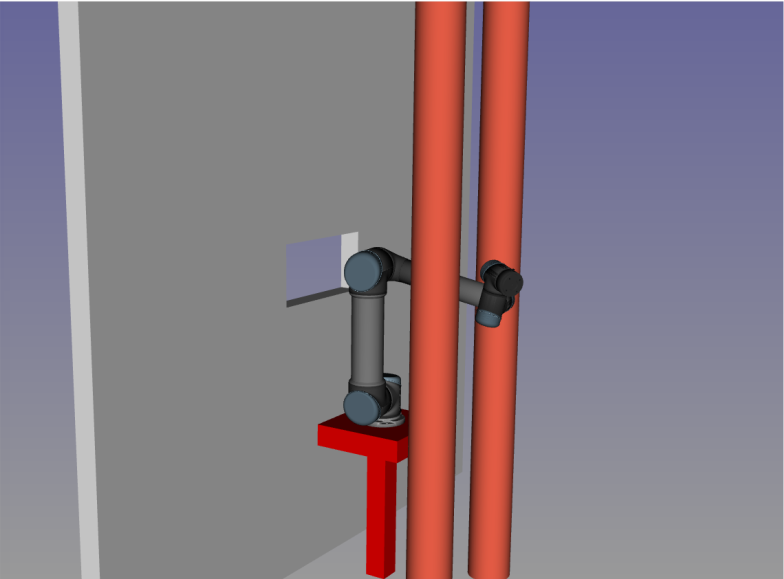
\includegraphics[width=\linewidth]{figures/motion-planning-init.png}
    }
    \centerline{initial configuration}
  }
  \parbox{.49\linewidth}{
    \centerline{
      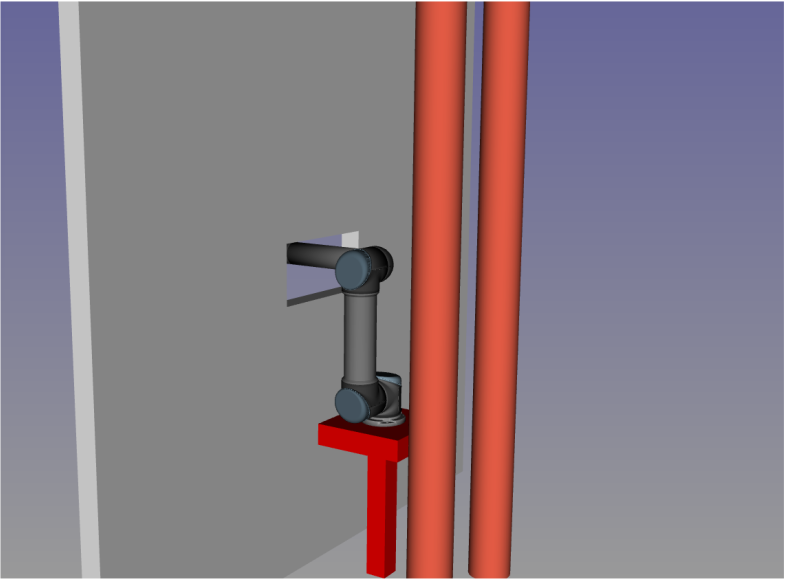
\includegraphics[width=\linewidth]{figures/motion-planning-goal.png}
    }
    \centerline{goal configuration}
  }
  \vskip .5cm
  \centerline{$\CS=\real^6$}
\end{frame}
